\documentclass{article}
\usepackage[utf8]{inputenc}
\usepackage{graphicx}
\usepackage{amsmath}
\usepackage{geometry}
\usepackage{hyperref}
\usepackage{minted}
\usepackage{subcaption}

\geometry{a4paper, margin=1in}

\title{Technical Report: Deep Reinforcement Learning for Humanoid Locomotion from an Image-Defined Initial Pose}
\author{Gemini Agent \\ on behalf of the project owner}
\date{\today}

\begin{document}

\maketitle

\begin{abstract}
This report details the implementation of an end-to-end pipeline that enables a simulated humanoid agent to learn stable walking using Deep Reinforcement Learning (DRL). The system's novelty lies in its ability to initialize the agent's starting pose for each training episode from a 25-keypoint skeleton extracted from a user-provided static image. This document covers the two main implemented modules: (1) Pose Estimation and Initial Pose Extraction, which processes an image to derive joint angles, and (2) the Simulation Environment, a custom Gymnasium-compliant physics world that uses these angles to pose a humanoid model. We also detail the implementation of the foundational reward system, which prepares the project for the final DRL agent training phase.
\end{abstract}

\section{Introduction}
The primary objective of this project is to develop a robust DRL-based walking policy for a simulated humanoid robot. A key challenge in humanoid locomotion is generalization across different starting conditions. This project addresses this by creating a system that can interpret a human pose from a static image, translate it into a corresponding configuration for a simulated humanoid, and then use that as the starting point for a learning episode. This approach aims to create a more versatile and robust walking gait. The project is divided into three main modules, of which the first two and the foundational elements of the third have been completed.

\section{Module 1: Pose Estimation & Initial Pose Extraction}
This module is responsible for processing a user-provided image, detecting human figures, extracting a skeletal representation, and converting that skeleton into a set of joint angles for the simulation.

\subsection{Image Acquisition and Preprocessing}
\textbf{File:} \texttt{humanoid_library/pose_estimation/imgAcquisition.py}

The first step in the pipeline is to load and prepare the input image.

\begin{itemize}
    \item \texttt{load_image(file_path)}: This function uses OpenCV (\texttt{cv2}) to read an image from a given file path. The image is immediately converted from the default BGR color space to RGB. Crucially, the image data type is converted from \texttt{uint8} to \texttt{np.float32} and pixel values are normalized from the [0, 255] range to [0.0, 1.0]. This is a standard preprocessing step for most deep learning models.
    
    \item \texttt{preprocess_image(image, target_size)}: To ensure consistent input size for the pose estimation model, this function resizes the image to a specified target size (e.g., 256x256 pixels) using OpenCV's resize functionality.
\end{itemize}

\subsection{Multi-Person 25-Keypoint Extraction}
\textbf{File:} \texttt{humanoid_library/pose_estimation/keyPointExtraction.py}

Once the image is preprocessed, the core pose detection takes place.

\begin{itemize}
    \item \textbf{Design Choice - MediaPipe vs. OpenPose:} The project specification mentions OpenPose and its BODY_25 model. However, a deliberate design choice was made to use Google's MediaPipe (\texttt{mediapipe}) library instead. This decision was motivated by ease of installation for the end-user, as MediaPipe is a simple \texttt{pip} installable package, whereas OpenPose often requires complex dependencies and compilation.
    
    \item \texttt{PoseExtractor} Class: This class encapsulates the pose detection logic.
    \begin{itemize}
        \item \texttt{\textbf{\textunderscore\textunderscore init\textunderscore\textunderscore()}}: The constructor initializes the MediaPipe Pose model (\texttt{mp.solutions.pose.Pose}). The model is configured for high accuracy (\texttt{model_complexity=2}) on static images.
        
        \item \texttt{\textbf{extract_keypoints(image)}}: This is the primary method of the class. It takes the preprocessed image, un-normalizes it back to the 0-255 range, and passes it to the MediaPipe detector. MediaPipe returns a set of 33 landmarks. To approximate the BODY_25 skeleton structure, a conversion process is applied:
        \begin{itemize}
            \item Some keypoints, like the nose and shoulders, are mapped directly.
            \item Other keypoints, such as the 'Neck' and 'MidHip', are not present in the MediaPipe output and are therefore calculated by averaging the positions of adjacent landmarks (e.g., Neck is the average of the left and right shoulder points).
        \end{itemize}
        The final output is a NumPy array of shape (25, 3), where each row represents a keypoint with (x, y, visibility) coordinates.
        
        \item \texttt{\textbf{draw_skeleton(image, skeleton_points, save_path)}}: A utility function for visualization. It draws the detected 25 keypoints and the connecting "bones" onto the original image, which is invaluable for debugging and verifying the accuracy of the pose extraction.
    \end{itemize}
\end{itemize}

\subsection{Target Selection and Kinematic Conversion}
\textbf{File:} \texttt{humanoid_library/pose_estimation/kinematicConversion.py}

With a skeleton extracted, it must be converted into a format the physics simulation can understand.

\begin{itemize}
    \item \texttt{select_main_skeleton_multiple(...)}: This function addresses the challenge of multiple people in an image. It runs the keypoint extraction process multiple times and selects the skeleton that occupies the largest bounding box area. This heuristic is effective for choosing the most prominent person in the frame.
    
    \item \texttt{compute_joint_angles(skeleton)}: This is the core of the kinematic conversion. It transforms the 2D Cartesian coordinates of the skeleton into a vector of 9 relative joint angles. The process is as follows:
    \begin{enumerate}
        \item \textbf{Vector Definition:} For each limb, a 2D vector is calculated by subtracting the coordinates of the two joints that define it (e.g., the right thigh vector \texttt{v_r_thigh} is computed from the right hip and right knee keypoints). A reference "up" vector is also defined based on the spine.
        \item \textbf{Angle Calculation:} The \texttt{numpy.arctan2(y, x)} function is used to calculate the angle of each limb vector relative to a reference vector. For instance, the right hip angle is the angle between the downward spine vector and the right thigh vector. This method correctly handles angles in all four quadrants.
        \item \textbf{Output:} The function returns a NumPy array containing 9 floating-point values, representing the angles (in radians) for the right/left hip, knee, shoulder, elbow, and the spine.
    \end{enumerate}
\end{itemize}

\section{Module 2: Simulation (Physics Environment)}
This module provides a physically accurate, controllable humanoid model within a custom environment that can be initialized to the specific pose derived in Module 1.

\subsection{Environment Instantiation and API}
\textbf{File:} \texttt{humanoid_library/simulation/humanoid_env.py}

The \texttt{HumanoidWalkEnv} class, which inherits from \texttt{gymnasium.Env}, manages the entire simulation state.

\begin{itemize}
    \item \texttt{\textbf{\textunderscore\textunderscore init\textunderscore\textunderscore()}}: The constructor sets up the simulation client using PyBullet, either in \texttt{GUI} mode for visualization or \texttt{DIRECT} mode for faster, headless training. It configures gravity and sets the search path to locate PyBullet's default assets. The environment's action space (17 continuous values for joint torques) and observation space (58 dimensions including joint states, torso position, and orientation) are defined.
    
    \item \texttt{\textbf{reset(initial_pose=None)}}: This key function prepares the environment for a new episode. It resets the PyBullet simulation, loads a ground plane, and then:
    \begin{enumerate}
        \item Calls \texttt{\_load_robot()} to load the \texttt{humanoid_symmetric.xml} MJCF model.
        \item Calls \texttt{\_get_actuated_joints()} to identify the controllable joints.
        \item If an \texttt{initial_pose} vector (from Module 1) is provided, it calls \texttt{\_apply_initial_pose()} to set the humanoid's starting configuration.
    \end{enumerate}
    It returns the first observation of the episode.
    
    \item \texttt{\textbf{\_apply_initial_pose(initial_pose)}}: This function is critical for bridging the gap between the 9-angle vector from pose estimation and the 17-joint humanoid model. A \texttt{joint_mapping} dictionary explicitly links each of the 9 angles to the correct joint index and axis in the simulation. For example, it maps the computed right hip angle (index 0 in our vector) to the humanoid's 'right_hip_y' joint (index 7 in the simulation). It then iterates through this mapping and uses \texttt{pybullet.resetJointState} to set each joint to its target angle.
    
    \item \texttt{\textbf{step(action)}}: This function advances the simulation. It takes an action from the agent (a vector of torques), applies these forces to the humanoid's joints using \texttt{pybullet.setJointMotorControlArray}, and steps the physics engine forward. It then computes the reward and checks for termination conditions, returning the standard \texttt{(obs, reward, terminated, truncated, info)} tuple.
\end{itemize}

\section{Module 3: Control (DQN Agent) - Foundations}
While the full DQN agent and training loop are part of the next phase, the essential reward and termination systems, as specified in the project PDF, have been implemented within the environment, making it ready for training.

\subsection{Reward Function Engineering}
The reward function, implemented in \texttt{\_compute_reward()}, is designed to incentivize a stable, forward walking gait. It consists of three components:
\begin{itemize}
    \item \textbf{Forward Velocity Reward (\texttt{r_vel})}: A positive reward proportional to the forward velocity of the humanoid's torso. This is the primary driver for locomotion.
    \item \textbf{Alive Bonus (\texttt{r_live})}: A small, constant positive reward given at every timestep that the agent does not fall. This encourages the agent to stay upright for as long as possible.
    \item \textbf{Energy Penalty (\texttt{torque_penalty})}: A small negative reward proportional to the sum of squared torques applied. This discourages jerky, inefficient movements and encourages a smoother gait.
\end{itemize}
The total reward is the sum of these components: \( R_t = r_{vel} + r_{live} - torque_{penalty} \).

\subsection{Termination Condition}
The episode must end if the agent fails. This is handled by the \texttt{\_check_termination()} function, which monitors the height of the humanoid's torso. If the torso's z-coordinate drops below a threshold of 0.7 meters, it signifies that the agent has fallen, and the function returns \texttt{True}, terminating the episode.

\section{Visual Results and Verification}
To verify the pipeline's effectiveness, we performed a test run using a sample image. The following figures illustrate the key stages of the process, demonstrating the system's ability to handle real-world images and translate them into the simulation environment.

\begin{figure}[h!]
    \centering
    \begin{subfigure}[b]{0.48\textwidth}
        
\includegraphics[width=\textwidth]{Testing/test1.jpg}
        \caption{Input image containing a person in a distinct pose.}
        \label{fig:input_image}
    \end{subfigure}
    \hfill
    \begin{subfigure}[b]{0.48\textwidth}
        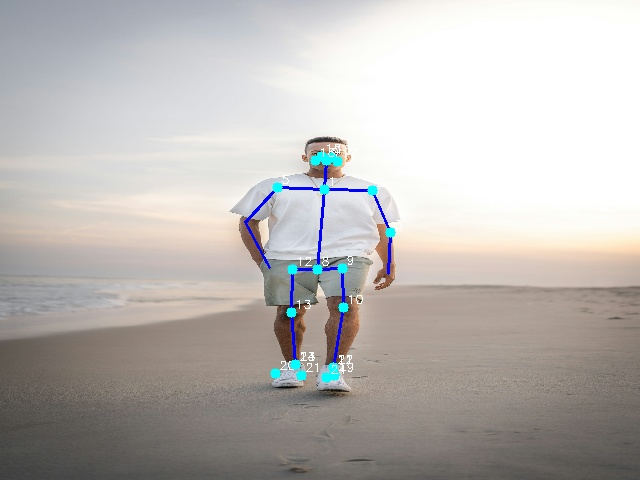
\includegraphics[width=\textwidth]{Testing/output_pose.jpg}
        \caption{The extracted 25-point skeleton is overlaid on the subject, showing the successful output of Module 1.}
        \label{fig:skeleton_output}
    \end{subfigure}
    \caption{Verification of the Pose Estimation and Extraction Pipeline.}
    \label{fig:pose_extraction}
\end{figure}

\begin{figure}[h!]
    \centering
    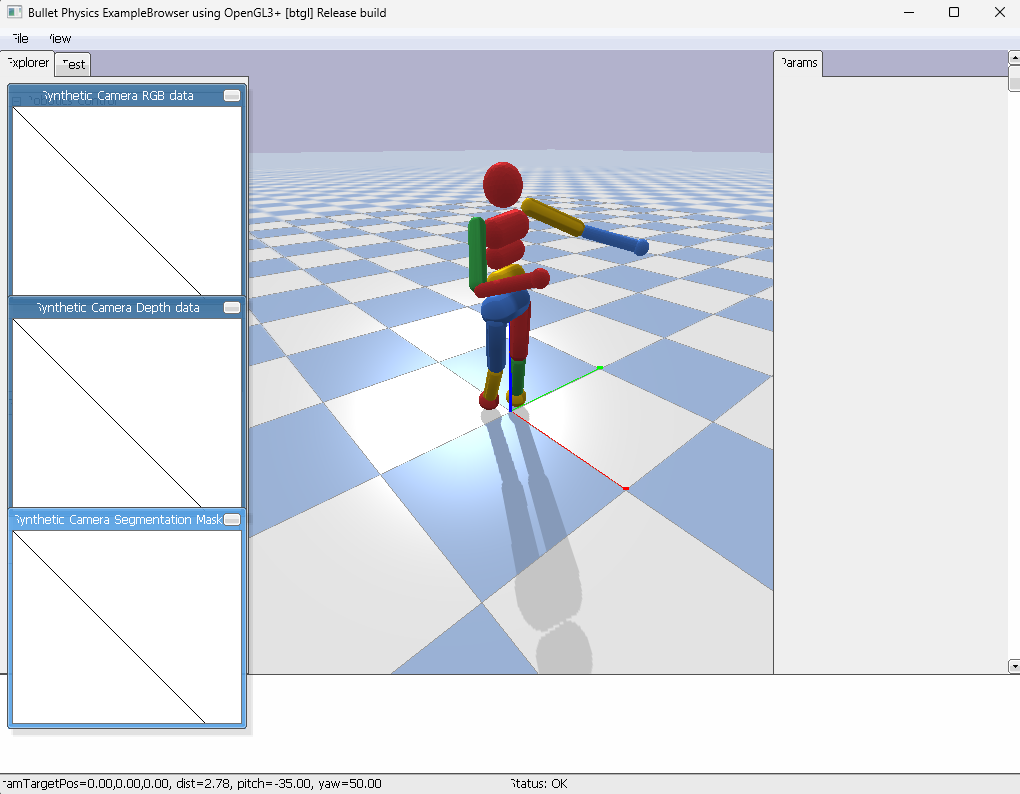
\includegraphics[width=0.6\textwidth]{Testing/humanoid_screenshot.png}
    \caption{The humanoid model rendered in the PyBullet simulation. Its pose is initialized based on the joint angles calculated from the extracted skeleton. The model is physically simulated, standing under gravity, ready to begin a learning episode.}
    \label{fig:humanoid_screenshot}
\end{figure}

\section{Conclusion and Future Work}
The work completed to date successfully establishes the full pipeline from image processing to a posed, reward-enabled simulation environment.
\begin{itemize}
    \item \textbf{Module 1 is complete:} The system can robustly load an image, extract a 25-point skeleton, and compute a 9-angle pose vector.
    \item \textbf{Module 2 is complete:} A custom Gymnasium environment can load a humanoid model and precisely set its initial pose based on the vector from Module 1.
    \item \textbf{Module 3 is initiated:} The foundational reward and termination functions described in the project plan have been implemented in the environment.
\end{itemize}
The project is now fully prepared for the final stage: the implementation of the Deep Q-Network (DQN) agent and the training loop that will teach the humanoid to walk from any given initial pose.

\end{document}
